\chapter{Análisis de los resultados obtenidos}\label{cp: results}
El algoritmo planteado fue entrenado con el dataset completo sin obtener resultados durante pocas épocas dado el elevado tiempo de entrenamiento por época. La precisión en entrenamiento no aumentaba con el paso de las épocas y se decidió reducir la complejidad del problema. Para ello, se entrenó el algoritmo con dos grabaciones de audio y se validó para una única grabación de audio. El algoritmo se entrenó con las siguientes características:
\begin{itemize}
	\item \textbf{Tamaño de batch}\arrowTikz{0}32
	\item \textbf{Número de \glspl{FFT}}
	\begin{itemize}
		\item Entrenamiento\arrowTikz{0}63132
		\item Validación\arrowTikz{0}4068
	\end{itemize}
	\item \textbf{Número de épocas}\arrowTikz{0}2000\footnote{El entrenamiento se paró en 1390 al comprobar que los resultados empeoraban}
	\item \textbf{Tasa de aprendizaje}\arrowTikz{0}Variable en el tiempo como muestra la gráfica \ref{fig: learning_rate}
\end{itemize}

\begin{figure}[h!]
	\centering
	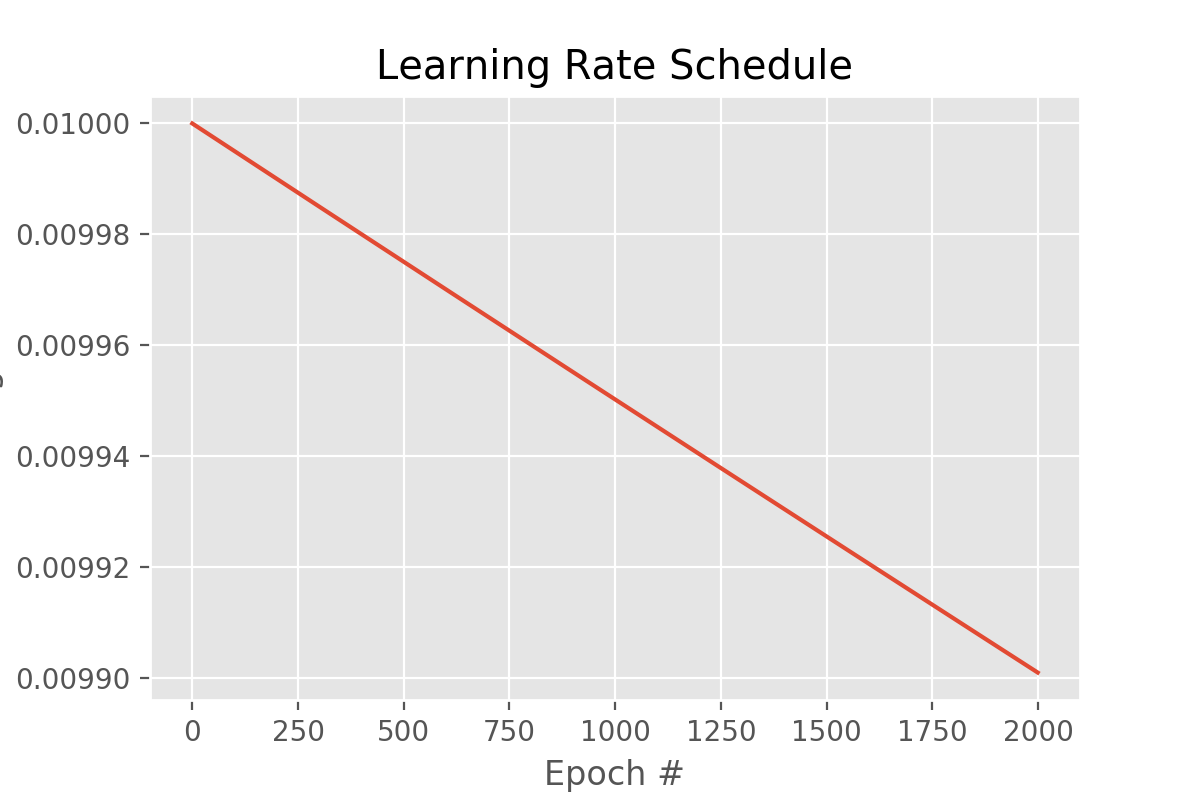
\includegraphics[width=0.75\columnwidth]{figures/Learning_rate_schedule}
	\caption{Variación de la tasa de aprendizaje con las épocas}
	\label{fig: learning_rate}
\end{figure}

Entrenado con esta configuración, el tiempo de entrenamiento por época es de 36 segundos con $\approx 569\mu$s por batch en una tarjeta gráfica \gls{AMD} Radeon Rx570 mediante el \gls{framework} \gls{ROCm}. 

Los resultados obtenidos distan mucho de un correcto funcionamiento. La precisión en entrenamiento se estabiliza en torno al 7\% y la precisión en validación llega al 2\% y decae hasta el 1\% claro síntoma de \textbf{overfitting} a pesar de tener una pobre precisión en entrenamiento.

\begin{figure}[h!]
	\centering
	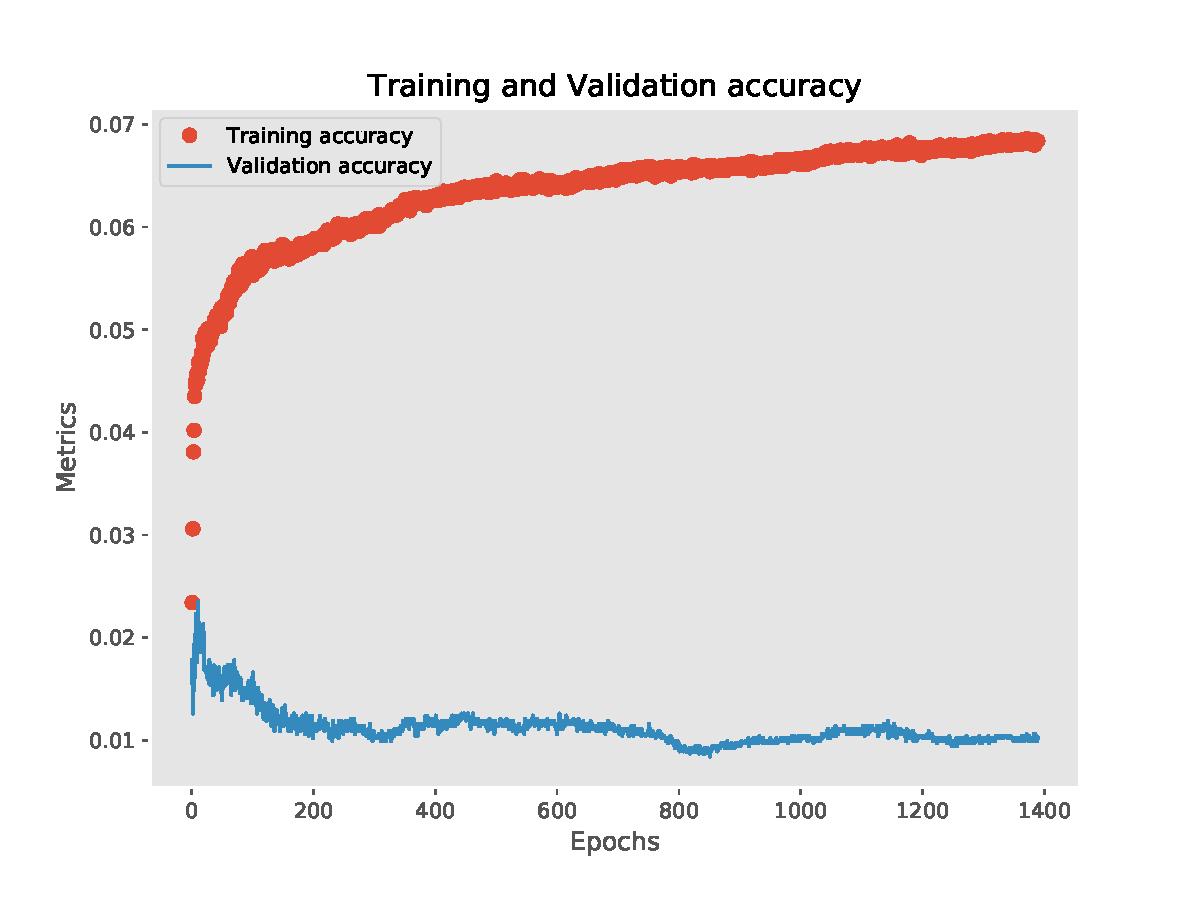
\includegraphics[width=0.75\columnwidth]{figures/one_to_one_results_acc.pdf}
	\caption{Precisión en entrenamiento y validación}
	\label{fig: results_acc}
\end{figure}
\begin{figure}[t!]
	\centering
	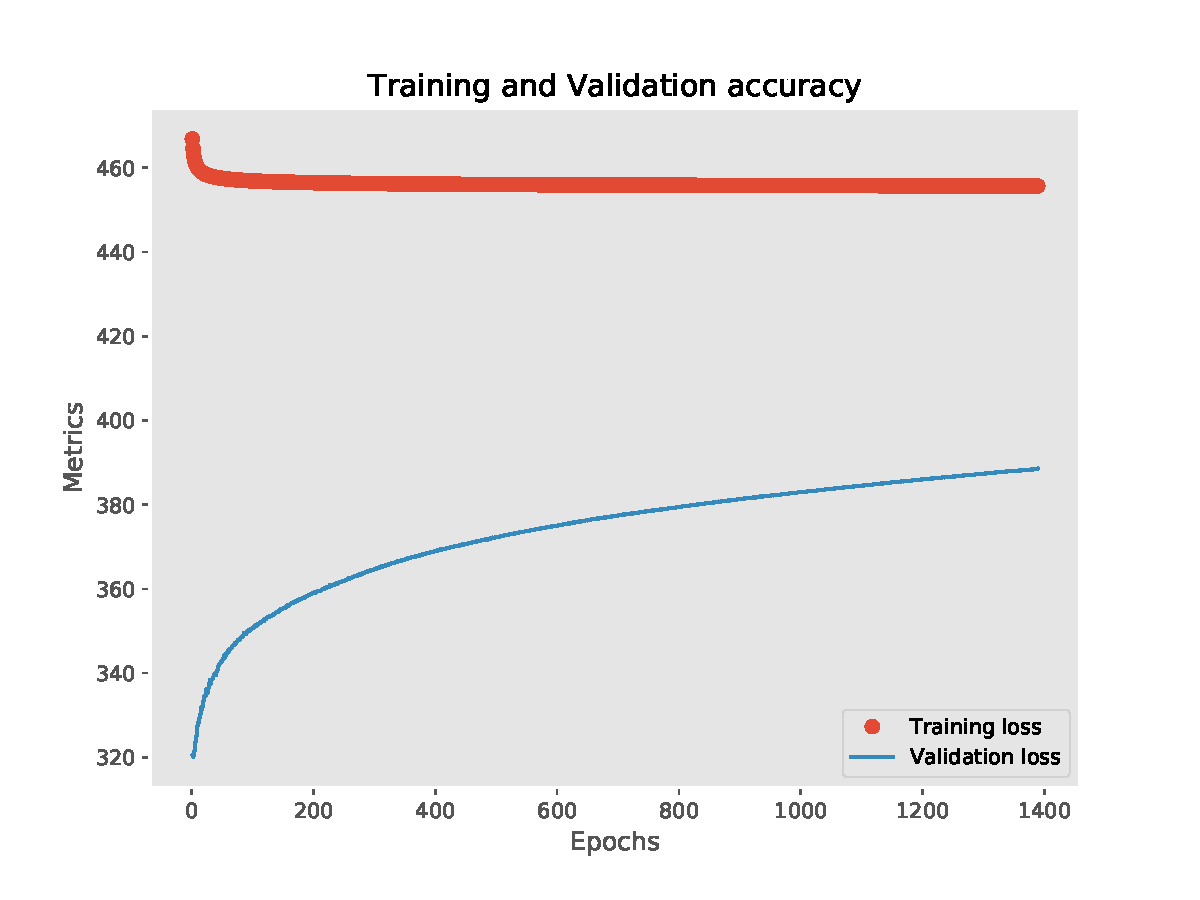
\includegraphics[width=0.75\columnwidth]{figures/one_to_one_results_loss.pdf}
	\caption{Pérdidas en entrenamiento y validación}
	\label{fig: results_loss}
\end{figure}

En las figuras \ref{fig: results_acc} y \ref{fig: results_loss} se puede ver las comparativas de pérdidas y precisión para entrenamiento y validación, respectivamente. En la gráficas se aprecia el claro overfitting. Algo a destacar es la lenta memorización de datos porque una red tan grande debería ser capaz de memorizar los datos de entrenamiento. Como se aprecia la precisión en entrenamiento no llega a una asíntota de modo que, idealmente debería continuar memorizando los datos con el paso de las épocas.

\section{Comparación con una red mono-capa}
Dada la escasez de precisión de los resultados obtenidos se decidió crear una red distinta con una sola capa \gls{LSTM}. Los resultados obtenidos fueron muy superiores y con 300 épocas para dos audios en entrenamiento y dos en validación los resultados continuaron mejorando pero a un ritmo ralentizado.

\begin{lstlisting}[basicstyle=\tiny\ttfamily, caption={Resumen del modelo mono-capa},captionpos=b, label={lst: model_resume_monolayer},frame=tb,
xleftmargin=.2\textwidth, xrightmargin=.2\textwidth]
_________________________________________________________________
Layer (type)                 Output Shape              Param #   
=================================================================
lstm (LSTM)                  (None, 2048)              18833408  
_________________________________________________________________
dense (Dense)                (None, 250)               512250    
=================================================================
Total params: 19,345,658
Trainable params: 19,345,658
Non-trainable params: 0
_________________________________________________________________
\end{lstlisting}

En \ref{lst: model_resume_monolayer} se tiene el modelo presentado en la comparación. Se trata de un modelo con muchos más parámetros pero más simple. Este modelo ha sido entrenado con los siguientes parámetros:

\begin{itemize}
	\item \textbf{Tamaño de batch}\arrowTikz{0}128
	\item \textbf{Número de \glspl{FFT}}
	\begin{itemize}
		\item Entrenamiento\arrowTikz{0}55657
		\item Validación\arrowTikz{0}11543
	\end{itemize}
	\item \textbf{Número de épocas}\arrowTikz{0}300\
	\item \textbf{Tasa de aprendizaje}\arrowTikz{0}Variable en el tiempo como muestra la gráfica \ref{fig: learning_rate_compa}
\end{itemize}

\begin{figure}[h!]
	\centering
	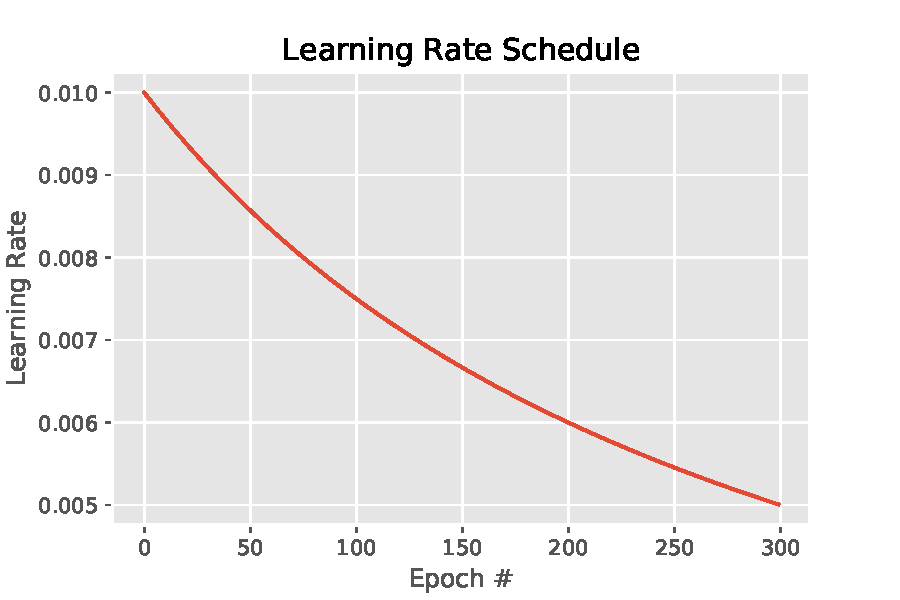
\includegraphics[width=0.75\columnwidth]{figures/Learning_rate_schedule_comparison}
	\caption{Variación de la tasa de aprendizaje con las épocas}
	\label{fig: learning_rate_compa}
\end{figure}

Los resultados obtenidos mejoran mucho a la red multi-capa siendo la red idónea para entrenar frente a un mayor abanico de audios y no una muestra reducida. La figura \ref{fig: results_acc_compa} muestra los resultados obtenidos y, aunque se ve cierto comportamiento asintótico en los resultados de validación, el algoritmo continúa mejorando en validación, aunque con una tasa reducida.
%\enlargethispage{0.5in}
%\vspace*{-50pt}
\begin{figure}[t!]
	\centering
	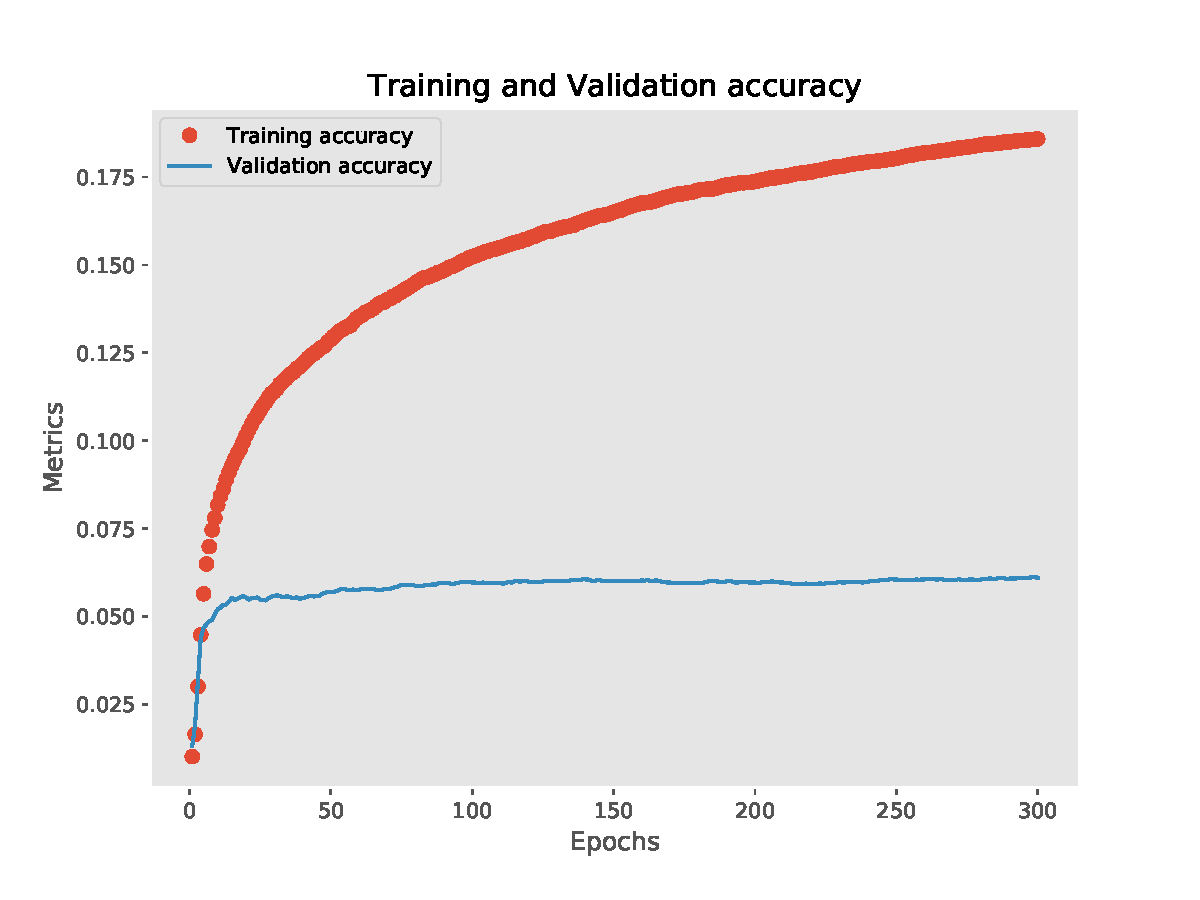
\includegraphics[width=0.75\columnwidth]{figures/results_acc_compa.pdf}
	\vspace*{-10pt}
	\caption{Precisión en entrenamiento y validación}
	\label{fig: results_acc_compa}
\end{figure}

Después de probar varios modelos, los resultados obtenidos con este último son los mejores dado que en entrenamiento continúa memorizando los datos, lo que da síntomas de que el tamaño de la red comienza a ser el adecuado. La precisión después de 300 épocas es del 18.5\% en entrenamiento frente al 7\% que da la red multi-capa menor (siendo ésta última entrenada en 1300 épocas) y en validación un 6\% frente a un 1\%.

El código relaciona con esta red se adjunta en \ref{lst: jupyter_notebook_proto} como un archivo de Jupyter Notebook dado que, para prototipado de arquitectura y dada la reducida cantidad de datos de entrenamiento (sobre la cual se prototipa), es la forma mejor de desarrollar. Una vez el algoritmo sea definitivo se le debe lanzar una batería mayor de entrenamiento, para ello se entrenaría con el generador de secuencias presentado en \ref{sec: sequence_gen}.